%\documentclass[pdf,notes]{beamer}
\documentclass[pdf,handout]{beamer}
\mode<presentation>{\usetheme[secheader]{Boadilla}}
\usepackage{mystyle}
\includecomment{versiona}
\usepackage{xeCJK}
\usepackage{subfig}

%\setbeameroption{hide notes}
\newcommand{\red}[1]{{\color[rgb]{0.6,0,0}#1}}
\setCJKmainfont[AutoFakeBold=true]{Hiragino Mincho Pro} %my Mac
%\setCJKmainfont{MS PGothic} %AJP windows

\makeatletter
\newenvironment<>{proofs}[1][\proofname]{\par\def\insertproofname{#1\@addpunct{.}}\usebeamertemplate{proof begin}#2}
{\usebeamertemplate{proof end}}
\makeatother

\makeatletter
\def\th@mystyle{%
\normalfont % body font
\setbeamercolor{block title example}{bg=orange,fg=white}
\setbeamercolor{block body example}{bg=orange!20,fg=black}
\def\inserttheoremblockenv{exampleblock}
}
\makeatother

\theoremstyle{mystyle}
\newtheorem{prop}{Proposition}

\renewcommand{\implies}{\Rightarrow}

\title{Hermitian Neural Networks}
\subtitle{joint with 小林俊行}
\author{レオンチエフ・アレックス、東大数理}

\begin{document}
\begin{frame}\titlepage\end{frame}
\begin{frame}{Outline}
\tableofcontents
\end{frame}
\newcommand{\mytime}[1]{(#1{分})}
\section{Intro: Orthogonal Neural Networks}
\begin{frame}
	\begin{figure}[h]
		\centering
		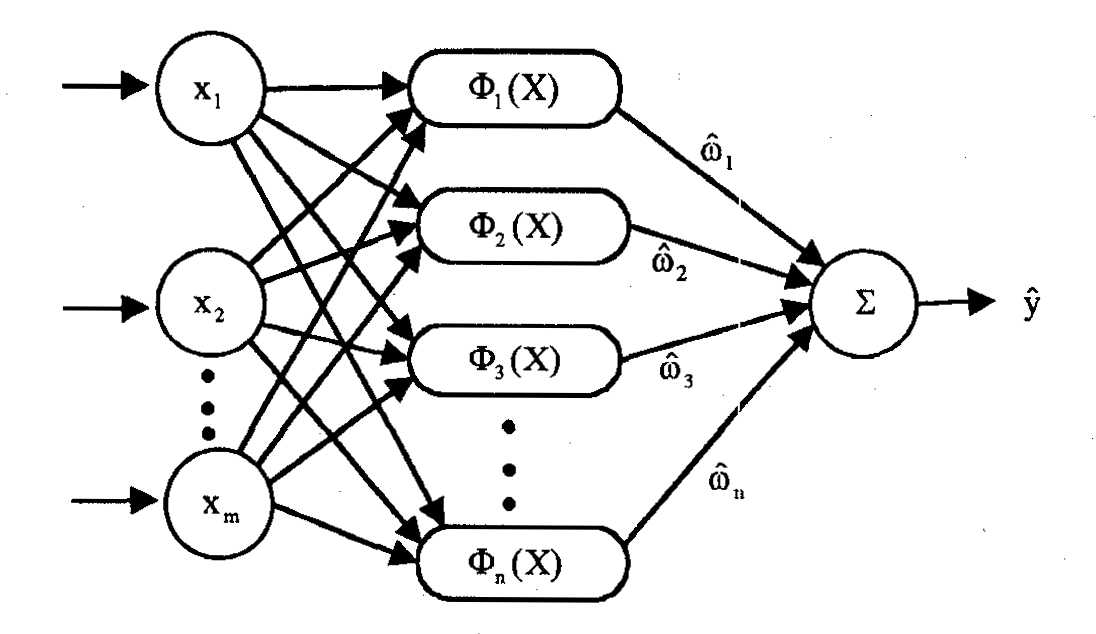
\includegraphics[scale=0.3]{onn}
		\caption{Orthogonal Neural Network (taken from \cite{yang1996orthogonal})}
		\label{fig:onn}
		%\note{tesime}
	\end{figure}
	\begin{block}{Idea}
		Approximate signal $y(x)$ using orthogonal functions:\begin{equation*}
			y(x)\approx \hat{y}(x):=\sum_{i=1}^N \hat{\omega}_i  \Phi_i(x)
		\end{equation*}
	\end{block}
	This connects neural networks with functional analysis!
\end{frame}
\begin{frame}{Advantages}
	\begin{itemize}
		\item Architecture is simple;\pause
		\item Parameters are few;\pause
		\item Can choose particular OFs to suit the particular problem domain (e.g. Hermite functions for medical imaging);\pause
		\item Error estimation is readily available ($\implies$ can estimate convergence speed);\pause
		\item For some OFs we can use recurrence relations to speed up the computation (e.g. Lagrange, Hermite functions/polynomials)
	\end{itemize}
\begin{figure}
  \centering
  \vspace{-0.6cm}
  \subfloat{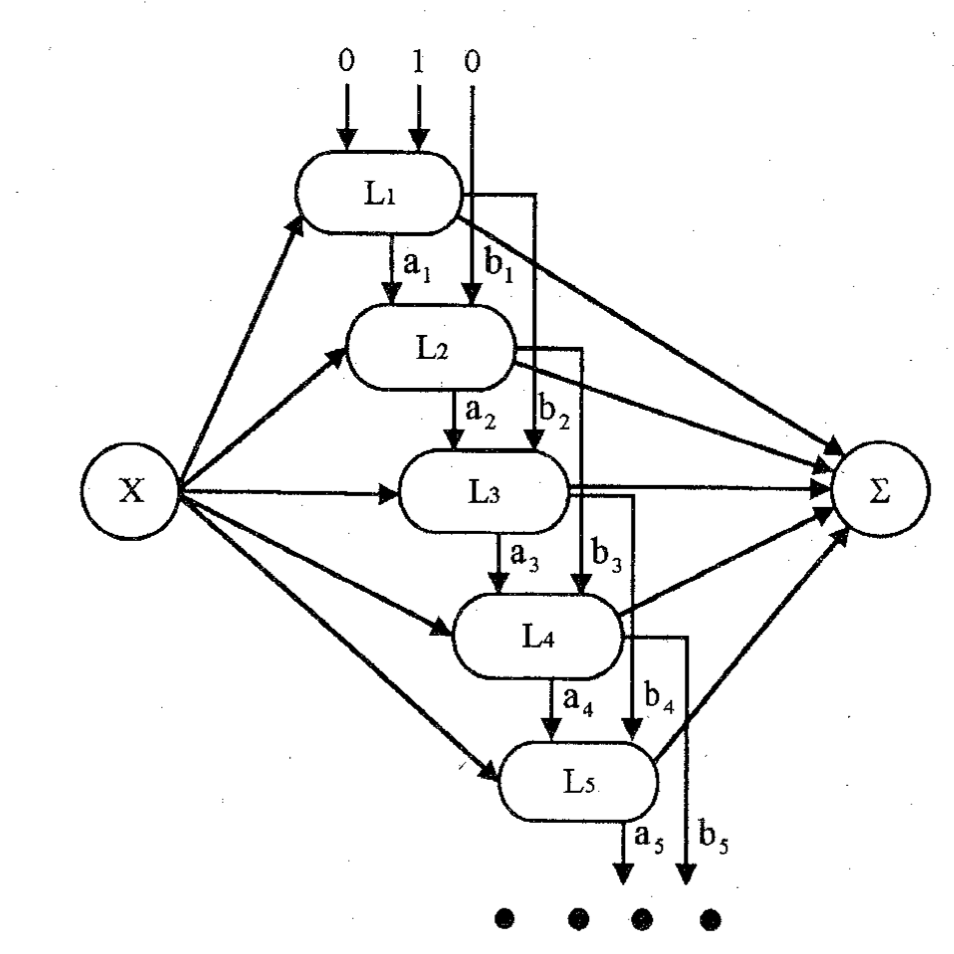
\includegraphics[scale=0.2]{onn2}}\qquad
  \subfloat{\raisebox{0.5cm}{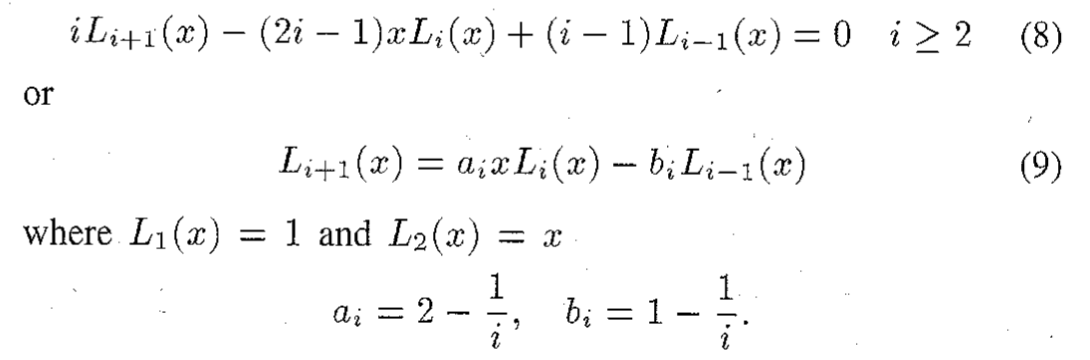
\includegraphics[scale=0.4]{onn3}}}
\caption{(taken from \cite{yang1996orthogonal})}
\end{figure}
\end{frame}
\section{Intro: Convolution of Hermitian Neural Networks}
\begin{frame}{Why Hermite Networks?}
	\begin{equation*}
		\begin{array}[]{c}
			h_n(t)=\frac{H_n(t)e^{-t^2/2}}{\sqrt{2^nn!\sqrt{\pi}}}\mbox{ (Hermite {\it functions})};\\
		H_n(t)=(-1)^n e^{t^2}\frac{d^n}{dt^n}e^{-t^2}\mbox{ (Hermite {\it polynomials})}.
		\end{array}
	\end{equation*}
	\pause
	\begin{itemize}
		\item Low order Hermite functions resemble some important signals in biomedical engineering \cite{mackenzie2003hermite};\pause
		\item Recursive formula $H_{n+1}(t)=2tH_n(t)-2nH_{n-1}(t)$ (see above);\pause
		\item Can be implemented in hardware \cite{mackenzie2003hermite};\pause
	\end{itemize}
	Besides, good analytic properties:\pause
	\begin{itemize}
		\item Invariant under Fourier transform: $\mathcal{F}(h_n)=\left( -i \right)^n\sqrt{2\pi}h_n$ $\left( \implies
			\mathcal{F}\left( \hat{y} \right)=\sum_{j=1}^N \hat{\omega}_j (-i)^j \sqrt{2\pi}h_j \right)$;
			\pause
		\item $h_0$ is Gaussian filter\vspace{-0.5cm}\begin{equation*}
				\implies e^{-t^2/2}\ast y\approx e^{-t^2/2} \ast \hat{y} =\sum_{i=1}^N \hat{\omega}_i \left( h_i\ast h_0 \right)
			\end{equation*}
			\vspace{-0.5cm}
	\end{itemize}
\end{frame}
\begin{frame}{Why Convolution?}
	We often need to convolve two Hermite Neural Networks (e.g. to recover noised signal with Gaussian):
	\begin{equation*}
		y_1\ast y_2\approx \hat{y}_1\ast \hat{y}_2=\sum_{i,j=1}^N a^{(1)}_i a^{\left( 2 \right)}_j \left(h_i\ast h_j  \right)
	\end{equation*}
	\pause
	It is good that we have an explicit formula:
	\begin{equation*}
		\left( h_i\ast h_j \right)(t)=\left\{\begin{array}[]{ll}
			\left( -1 \right)^{i+j}l_j^{i-j}\left( \frac{t^2}{2} \right),&t\ge0\\
			l_{j}^{i-j}\left( \frac{t^2}{2} \right),&t<0
		\end{array}\right.(j\le i).
	\end{equation*}
	\pause
	\begin{itemize}
		\item There are fast algorithms to compute special functions/polynomials (e.g. recursive relations);\pause
		\item Can do asymptotic analysis and error estimate very precise;
	\end{itemize}
\end{frame}
\section{Intro: Hermite-Rodriguez Networks}
\begin{frame}{Hermite-Rodriguez functions}
	We can repeat all of the above using Hermite-Rodriguez functions:
	\begin{equation*}
		hr_i(t)=\frac{h_i(t)e^{-t^2/2}}{\pi^{1/4}}=
		\frac{H_i(t)e^{-t^2}}{\sqrt{2^ii!{\pi}}}.
	\end{equation*}
	\pause For them we also have an explicit correlation formula
	\begin{equation}
		\left( hr_i\ast hr_j \right)(t)=\sqrt{\frac{(i+j)!}{2^{i+j}i!j!}}hr_{i+j}\left( \frac{t}{\sqrt{2}} \right).
		\label{eqn:HRcorrelation}
	\end{equation}
	\pause
	Hermitian-Rodriguez can be beneficial when analyzing high-frequency signals (e.g. glitches) \cite{mackenzie2003hermite}.
\end{frame}
\section{My contribution}
\begin{frame}{My contribution}
	The following holds:
	\begin{equation}
		  \int_{- 1}^1 \int_{- 1}^1 (1 - s^2)^{\lambda -
			    \frac{1}{2}} (1 - t^2)^{\mu - \frac{1}{2}} | s - t |^{- 2} d s d t
			    = \frac{- 2^{2\lambda+2\mu-1} \Gamma \left( \lambda + \frac{1}{2} \right)^2 \Gamma \left( \mu
			        + \frac{1}{2} \right)^2}{(\lambda + \mu - 1) \Gamma (2 \lambda) \Gamma (2
					  \mu)} .
		\label{eqn:2}
	\end{equation}
	\pause From here, we easily arrive at:\begin{equation}
		\int_{- 1}^1 \int_{- 1}^1 | s - t |^{2 \nu} (1 - s^2)^{\lambda - \frac{1}{2}}
		(1 - t^2)^{\mu - \frac{1}{2}} C_l^{\lambda} (s) C_m^{\mu} (t) d s d t=\dots
		\label{eqn:3}
	\end{equation}
\end{frame}
\begin{frame}
	Two more equivalent forms of $\eqref{eqn:3}$:\pause
	\begin{equation}
		\myabs{s-t}^{2 \nu} = \sum_{\ell, m = 0 \mid l + m : \mbox{even}}^{\infty}
		a_{\lambda, \mu, \nu}^{\ell, m} C_{\ell}^{\lambda} (s) C_m^{\mu} (t),
		\label{eqn:4}
	\end{equation}
	\begin{equation*}
 	a^{\ell,m}_{\lambda,\mu,\nu}=\dots,
	\end{equation*}
	\pause
	\begin{equation}
		\begin{array}{c}
			  \int_{- 1}^1 \int_{- 1 + s}^{1 + s} | w |^{2 \nu} c_m^{\mu} (s - w) \;
			    c^{\lambda}_l (s) \mbox{dwds} = \ldots,
		      \end{array}
		\label{eqn:5}
	\end{equation}
	\begin{equation*}
			      c^{\lambda}_l (s) = (1 - s^2)^{\lambda - \frac{1}{2}} C^{\lambda}_l (s).
	\end{equation*}
\end{frame}
\begin{frame}
	Taking limit in $\eqref{eqn:5}$ we arrive at
	\begin{equation*}
		\begin{array}{lccl}
			&\int_{-\infty}^\infty\myabs{w}^{2\nu}&\int_{-\infty}^\infty hr_m\left( s-w \right)hr_n(s)\mbox{ds\;dw}&=\dots\\\pause
			(\mbox{Mellin transform }\rightarrow)&\mathcal{M} &\left( hr_m\ast hr_n  \right)&=\dots
		\end{array}
	\end{equation*}
	\pause Using inverse Mellin transform (and a bit of magic) we can recover {\it convolution formula for Hermite-Rodriguez functions} $\eqref{eqn:HRcorrelation}$!\\
	\begin{equation*}
		\left( hr_i\ast hr_j \right)(t)=\sqrt{\frac{(i+j)!}{2^{i+j}i!j!}}hr_{i+j}\left( \frac{t}{\sqrt{2}} \right).
		\tag{(1)}
	\end{equation*}
\end{frame}
\section{Further work}
\begin{frame}{But we can do more!}
	\begin{enumerate}
		\item 
	\end{enumerate}
\end{frame}
\section{Q\&{A}\mytime{20}}
\begin{frame}
	\begin{center}
		\Huge Q\&{A}
	\end{center}
\end{frame}
\begin{frame}[allowframebreaks]
\frametitle{References}
\nocite{mackenzie2003hermite}
\nocite{yang1996orthogonal}
\bibliographystyle{apalike}
\bibliography{fmsp.bib}
\end{frame}
\end{document}
